% Copyright 2006 by Till Tantau
%
% This file may be distributed and/or modified
%
% 1. under the LaTeX Project Public License and/or
% 2. under the GNU Free Documentation License.
%
% See the file doc/generic/pgf/licenses/LICENSE for more details.


\section{Transparency}

\label{section-tikz-transparency}


\subsection{Overview}

Normally, when you paint something using any of \tikzname's commands
(this includes stroking, filling, shading, patterns, and images), the
newly painted objects totally obscure whatever was painted earlier in
the same area.

You can change this behaviour by using something that can be thought
of as ``(semi)transparent colors.'' Such colors do not completely
obscure the background, rather they blend the background with the new
color. At first sight, using such semitransparent colors might seem quite
straightforward, but the math going on in the background is quite
involved and the correct handling of transparency fills some 64 pages
in the PDF specification. 

In the present section, we start with the different ways of specifying
``how transparent'' newly drawn objects should be. The simplest way is
to just specify a percentage like ``60\% transparent.'' A much more
general way is to use something that I call a \emph{fading,} also
known as a soft mask or a mask.

At the end of the section we adress the problem of creating so-called
\emph{transparency groups}. This problem arises when you paint over a
position several times with a semitransparent color. Sometimes you
want the effect to accumulate, sometimes you do not.

\emph{Note:} Transparency is best supported by the pdf\TeX\
driver. The \textsc{svg} driver also has some support. For PostScript
output, opacity is rendered correctly only with the most recent
versions of GhostScript. Printers and other programs will typically
ignore the opacity setting. 



\subsection{Specifying a Uniform Opacity}

Specifying a stroke and/or fill opacity is quite easy using the
following options.


\begin{key}{/tikz/draw opacity=\meta{value}}
  This option sets ``how transparent'' lines should be. A value of |1|
  means ``fully opaque'' or ``not transparent at all,'' a value of |0|
  means ``fully transparent'' or ``invisible.'' A value of |0.5|
  yields lines that are semitransparent.

  Note that when you use PostScript as your output format,
  this option works only with recent versions of GhostScript.
   
\begin{codeexample}[]
\begin{tikzpicture}[line width=1ex]
  \draw (0,0) -- (3,1);
  \filldraw [fill=examplefill,draw opacity=0.5] (1,0) rectangle (2,1);
\end{tikzpicture}
\end{codeexample}
\end{key}

Note that the |draw opacity| options only sets the opacity of drawn
lines. The opacity of fillings is set using the option
|fill opacity| (documented in Section~\ref{section-fill-opacity}. The
option |opacity| sets both at the same time. 

\begin{key}{/tikz/opacity=\meta{value}}
  Sets both the drawing and filling opacity to \meta{value}.

  The following predefined styles make it easier to use this option:
  \begin{stylekey}{/tikz/transparent}
    Makes everything totally transparent and, hence, invisible.

\begin{codeexample}[]
\tikz{\fill[red]             (0,0)   rectangle (1,0.5);
      \fill[transparent,red] (0.5,0) rectangle (1.5,0.25); }
\end{codeexample}
  \end{stylekey}

  \begin{stylekey}{/tikz/ultra nearly transparent}
    Makes everything, well, ultra nearly transparent.

\begin{codeexample}[]
\tikz{\fill[red]                      (0,0)   rectangle (1,0.5);
      \fill[ultra nearly transparent] (0.5,0) rectangle (1.5,0.25); }
\end{codeexample}
  \end{stylekey}

  \begin{stylekey}{/tikz/very nearly transparent}
\begin{codeexample}[]
\tikz{\fill[red]                     (0,0)   rectangle (1,0.5);
      \fill[very nearly transparent] (0.5,0) rectangle (1.5,0.25); }
\end{codeexample}
  \end{stylekey}

  \begin{stylekey}{/tikz/nearly transparent}
\begin{codeexample}[]
\tikz{\fill[red]                (0,0)   rectangle (1,0.5);
      \fill[nearly transparent] (0.5,0) rectangle (1.5,0.25); }
\end{codeexample}
  \end{stylekey}

  \begin{stylekey}{/tikz/semitransparent} 
\begin{codeexample}[]
\tikz{\fill[red]             (0,0)   rectangle (1,0.5);
      \fill[semitransparent] (0.5,0) rectangle (1.5,0.25); }
\end{codeexample}
  \end{stylekey}

  \begin{stylekey}{/tikz/nearly opaque}   
\begin{codeexample}[]
\tikz{\fill[red]           (0,0)   rectangle (1,0.5);
      \fill[nearly opaque] (0.5,0) rectangle (1.5,0.25); }
\end{codeexample}
  \end{stylekey}
 
  \begin{stylekey}{/tikz/very nearly opaque} 
\begin{codeexample}[]
\tikz{\fill[red]                (0,0)   rectangle (1,0.5);
      \fill[very nearly opaque] (0.5,0) rectangle (1.5,0.25); }
\end{codeexample}
  \end{stylekey}

  \begin{stylekey}{/tikz/ultra nearly opaque}
\begin{codeexample}[]
\tikz{\fill[red]                 (0,0)   rectangle (1,0.5);
      \fill[ultra nearly opaque] (0.5,0) rectangle (1.5,0.25); }
\end{codeexample}
  \end{stylekey}

  \begin{stylekey}{/tikz/opaque}
    This yields completely opaque drawings, which is the default.
\begin{codeexample}[]
\tikz{\fill[red]    (0,0)   rectangle (1,0.5);
      \fill[opaque] (0.5,0) rectangle (1.5,0.25); }
\end{codeexample}
  \end{stylekey}
\end{key}


\begin{key}{/tikz/fill opacity=\meta{value}}
  This option sets the opacity of fillings. In addition to filling
  operations, this opacity also applies to text and images.

  Note, again, that when you use PostScript as your output format,
  this option works only with recent versions of GhostScript.
  
\begin{codeexample}[]
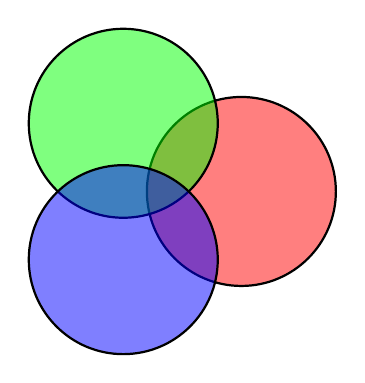
\begin{tikzpicture}[thick,fill opacity=0.5]
  \filldraw[fill=red]   (0:1cm)    circle (12mm);
  \filldraw[fill=green] (120:1cm)  circle (12mm);
  \filldraw[fill=blue]  (-120:1cm) circle (12mm);
\end{tikzpicture}
\end{codeexample}

\begin{codeexample}[]
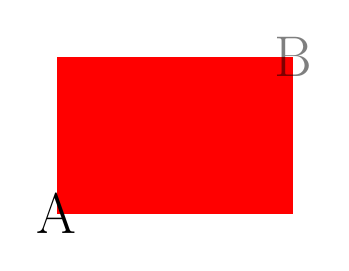
\begin{tikzpicture}
  \fill[red] (0,0) rectangle (3,2);

  \node                   at (0,0) {\huge A};
  \node[fill opacity=0.5] at (3,2) {\huge B};
\end{tikzpicture}
\end{codeexample}
\end{key}

\begin{key}{/tikz/text opacity=\meta{value}}
  Sets the opacity of text labels, overriding the |fill opacity| setting. 
\begin{codeexample}[]
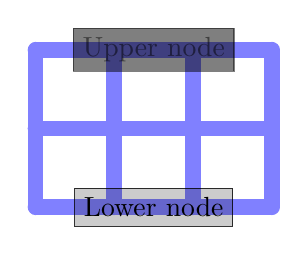
\begin{tikzpicture}[every node/.style={fill,draw}]
  \draw[line width=2mm,blue!50,cap=round] (0,0) grid (3,2);

  \node[opacity=0.5] at (1.5,2) {Upper node};
  \node[draw opacity=0.8,fill opacity=0.2,text opacity=1]
    at (1.5,0) {Lower node};
\end{tikzpicture}
\end{codeexample}
\end{key}


Note the following effect: If you setup a certain opacity for stroking
or filling and you stroke or fill the same area twice, the effect
accumulates:

\begin{codeexample}[]
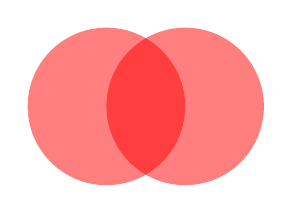
\begin{tikzpicture}[fill opacity=0.5]
  \fill[red] (0,0) circle (1);
  \fill[red] (1,0) circle (1);
\end{tikzpicture}
\end{codeexample}

Often, this is exactly what you intend, but not always. You can use
transparency groups, see the end of this section, to change this.


\subsection{Fadings}

For complicated graphics, uniform transparency settings are not always
sufficient. Suppose, for instance, that while you paint a picture, you
want the transparency to vary smoothly from completely opaque to
completely transparent. This is a ``shading-like'' transparency. For
such a form of transparency I will use the term \emph{fading} (as a
noun). They are also known as \emph{soft masks}, \emph{opacity masks},
\emph{masks}, or \emph{soft clips}.


\subsubsection{Creating Fadings}

How do we specify a fading? This is a bit of an art since the
underlying mechanism is quite powerful, but a bit difficult to use.

Let us start with a bit of terminology. A \emph{fading} specifies for
each point of an area to transparency of the point. This transparency
can by any number between 0 and 1. A \emph{fading picture} is a normal
graphic that, in a way to be described in a moment, determines the
transparency of points inside the fading. Each fading has an
underlying fading picture. 

The fading picture is a normal graphic drawn using any of the normal
graphic drawing commands. A fading and its fading picture are related
as follows: Given any point of the fading, the transparency of this
point is determined by the lumonisity of the fading picture at the
same position. The luminosity of a point determines ``how bright'' the
point is. The brighter the point in the fading picture, the more
opaque is the point in the fading. In particular, a white point of the
fading picture is completely opaque in the fading and a black point of
the fading picture is completely transparent in the fading. (The
background of the fading picture is always transparent in the fading
as if the background where black.)

It is rather counter-intuitive that a \emph{white} pixel of the fading
picture will be \emph{opaque} in the fading and a \emph{black} pixel
will be \emph{transparent}. For this reason, \tikzname\ defines a
color called |transparent| that is the same as |black|. The nice thing
about this definition is that the color
|transparent!|\meta{percentage} in the fading picture yields a
pixel that is \meta{percantage} per cent transparent in the fading. 

Turning a fading picture into a normal picture is achieved using the
following commands, which are \emph{only defined in the library},
namely the library |fadings|. So, to use them, you have to say
|\usetikzlibrary{fadings}| first.

\begin{environment}{{tikzfadingfrompicture}\oarg{options}}
  This command works like a |{tikzpicture}|, only the picture is not
  shown, but instead a fading is defined based on this picture. To set
  the name of the picture, use the |name| option (which is normally
  used to set the name of a node).
  \begin{key}{/tikz/name=\marg{name}}
    Use this option with the |{tikzfadingfrompicture}| environment to
    set the name of the fading. You \emph{must} provide this option.
  \end{key}
  
  The following shading is 2cm by 2cm and changes gets more and more
  transparent from left to right, but is 50\% transparent for a large
  circle in the middle.
\begin{codeexample}[]
\begin{tikzfadingfrompicture}[name=fade right]
  \shade[left color=transparent!0,
         right color=transparent!100] (0,0) rectangle (2,2);
  \fill[transparent!50] (1,1) circle (0.7);
\end{tikzfadingfrompicture}

% Now we use the fading in another picture:
\begin{tikzpicture}
  % Background
  \fill [black!20] (-1.2,-1.2) rectangle (1.2,1.2);
  \pattern [pattern=checkerboard,pattern color=black!30]
                   (-1.2,-1.2) rectangle (1.2,1.2);
  
  \fill [path fading=fade right,red] (-1,-1) rectangle (1,1);
\end{tikzpicture}
\end{codeexample}
  In the next example we create a fading picture that contains some
  text. When the fading is used, we only see the shading ``through
  it.'' 
\begin{codeexample}[]
\begin{tikzfadingfrompicture}[name=tikz]
  \node [text=transparent!20]
    {\fontfamily{ptm}\fontsize{45}{45}\bfseries\selectfont Ti\emph{k}Z};
\end{tikzfadingfrompicture}

% Now we use the fading in another picture:
\begin{tikzpicture}
  \fill [black!20] (-2,-1) rectangle (2,1);
  \pattern [pattern=checkerboard,pattern color=black!30]
                   (-2,-1) rectangle (2,1);

  \shade[path fading=tikz,fit fading=false,
         left color=blue,right color=black]
    (-2,-1) rectangle (2,1);
\end{tikzpicture}
\end{codeexample}
\end{environment}

\begin{plainenvironment}{{tikzfadingfrompicture}\oarg{options}}
  The plain\TeX\ version of the environment.
\end{plainenvironment}

\begin{contextenvironment}{{tikzfadingfrompicture}\oarg{options}}
  The Con\TeX t version of the environment.
\end{contextenvironment}

\begin{command}{\tikzfading\oarg{options}}
  This command is used to define a fading similarly to that way a
  shading is defined. In the \meta{options} you should 
  \begin{enumerate}
  \item use the |name=|\meta{name} option to set a name for the fading,
  \item use the |shading| option to set the name of the shading that
    you wish to use,
  \item extra options for setting the colors of the shading (typically
    you will set them to the color |transparent!|\meta{percentage}).
  \end{enumerate}
  Then, a new fading named \meta{name} will be created based on the
  shading.

\begin{codeexample}[]
\tikzfading[name=fade right,
            left color=transparent!0,
            right color=transparent!100]

% Now we use the fading in another picture:
\begin{tikzpicture}
  % Background
  \fill [black!20] (-1.2,-1.2) rectangle (1.2,1.2);
  \path [pattern=checkerboard,pattern color=black!30]
                   (-1.2,-1.2) rectangle (1.2,1.2);

  \fill [red,path fading=fade right] (-1,-1) rectangle (1,1);
\end{tikzpicture}
\end{codeexample}  

\begin{codeexample}[]
\tikzfading[name=fade out,
            inner color=transparent!0,
            outer color=transparent!100]

% Now we use the fading in another picture:
\begin{tikzpicture}
  % Background
  \fill [black!20] (-1.2,-1.2) rectangle (1.2,1.2);
  \path [pattern=checkerboard,pattern color=black!30]
                   (-1.2,-1.2) rectangle (1.2,1.2);

  \fill [blue,path fading=fade out] (-1,-1) rectangle (1,1);
\end{tikzpicture}
\end{codeexample}  
\end{command}



\subsubsection{Fading a Path}

Aa fading specifies for each pixel of a certain area how transparent
this pixel will be. The following options are used to install such a
fading for the current scope or path. 

\pgfdeclarefading{fade down}{%
  \tikzset{top color=pgftransparent!0,bottom color=pgftransparent!100}
  \pgfuseshading{axis}
}
\pgfdeclarefading{fade inside}{%
  \tikzset{inner color=pgftransparent!90,outer color=pgftransparent!30}
  \pgfuseshading{radial}
}

\begin{key}{/tikz/path fading=\meta{name} (default \normalfont scope's setting)}
  This option tells \tikzname\ that the current path should be faded
  with the fading \meta{name}. If no \meta{name} is given, the 
  \meta{name} set for the whole scope is used. Similarly to options
  like |draw| or |fill|, this option is reset for each path, so you
  have to add it to each path that should be faded. You can also
  specify |none| as \meta{name}, in which case fading for the path
  will be switched off in case it has been switched on by previous
  options or styles.
\begin{codeexample}[]
\begin{tikzpicture}[path fading=south]
  % Checker board
  \fill [black!20] (0,0) rectangle (4,3);
  \pattern [pattern=checkerboard,pattern color=black!30]
                   (0,0) rectangle (4,3);

  \fill [color=blue]                   (0.5,1.5) rectangle +(1,1);
  \fill [color=blue,path fading=north] (2.5,1.5) rectangle +(1,1);

  \fill [color=red,path fading]        (1,0.75) ellipse (.75 and .5);
  \fill [color=red]                    (3,0.75) ellipse (.75 and .5);
\end{tikzpicture}
\end{codeexample}

  \begin{key}{/tikz/fit fading=\meta{boolean} (default true, initially true)}
    When set to |true|, the fading is shifted and resized (in exactly
    the same way as a shading) so that is covers the current
    path. When set to |false|, the fading is only shifted so that it
    is centered on the path's center, but it is not resized. This can
    be useful for special-purpose fadings, for instance when you use a
    fading to ``punsh out'' something.
  \end{key}

  \begin{key}{/tikz/fading transform=\meta{transformation options}}
    The \meta{transformation options} are applied to the fading before
    it is used. For instance, if \meta{transformation options} is set
    to |rotate=90|, the fading is rotated by 90 degrees.
\begin{codeexample}[]
\begin{tikzpicture}[path fading=fade down]
  % Checker board
  \fill [black!20] (0,0) rectangle (4,1.5);
  \path [pattern=checkerboard,pattern color=black!30] (0,0) rectangle (4,1.5);

  \fill [red,path fading,fading transform={rotate=90}]
    (1,0.75) ellipse (.75 and .5);
  \fill [red,path fading,fading transform={rotate=30}]
    (3,0.75) ellipse (.75 and .5);
\end{tikzpicture}
\end{codeexample}
  \end{key}
  
  \begin{key}{/tikz/fading angle=\meta{degree}}
    A shortcut for |fading transform={rotate=|\meta{degree}|}|.
  \end{key}

  Note that you can ``fade just about anything.'' In particular, you
  can fade a shading.
  
\begin{codeexample}[]
\begin{tikzpicture}
  % Checker board
  \fill [black!20] (0,0) rectangle (4,4);
  \path [pattern=checkerboard,pattern color=black!30] (0,0) rectangle (4,4);

  \shade [ball color=blue,path fading=south] (2,2) circle (1.8);
\end{tikzpicture}
\end{codeexample}

  The |fade inside| of the following example more transparent in the middle than on the
  outside.

\begin{codeexample}[]
\tikzfading[name=fade inside,
            inner color=transparent!80,
            outer color=transparent!30]    
\begin{tikzpicture}
  % Checker board
  \fill [black!20] (0,0) rectangle (4,4);
  \path [pattern=checkerboard,pattern color=black!30] (0,0) rectangle (4,4);

  \shade [ball color=red] (3,3) circle (0.8);
  \shade [ball color=white,path fading=fade inside] (2,2) circle (1.8);
\end{tikzpicture}
\end{codeexample}

  Note that adding the |path fading| option to a node fades the
  (background) path, not the text itself. To fade the text, you need
  to use a scope fading (see below).
\end{key}



\subsubsection{Fading a Scope}

In addtion to fading individual paths, you may also wish to ``fade a
scope,'' that is, you may wish to install a fading that is used
globally to specify the transparency for all objects drawn inside a
scope. This effect can also be thought of as a ``soft clip'' and it
works in a similar way: You add the |scope fading| option to a path in
a scope -- typically the first one -- and then all subsequent drawings
in the scope are faded. You will use a |transparency group| in
conjunction, see the end of this section.

\begin{key}{/tikz/scope fading=\meta{fading}}
  In principle, this key works in excatly the same way as the
  |path fading| key. The only difference is, that the effect of the
  fading will persist after the current path till the end of the
  scope. Thus, the \meta{fading} is applied to all subsequent drawings
  in the current scope, not just to the current path. In this regard,
  the option works very much like the |clip| option. (Note, however,
  that, unlike the |clip| option, fadings to not accumulate unless a
  transparency group is used.)

  The keys |fit fading| and |fading transform| have the same effect as
  for |path fading|. Also that, just as for |path fading|, providing
  the |scope fading| option with a |{scope}| only sets the name of the
  fading to be used. You have to explicitly provide the |scope fading|
  with a path to actually install a fading.
  
\begin{codeexample}[]
\begin{tikzpicture}
  \fill [black!20] (-2,-2) rectangle (2,2);
  \pattern [pattern=checkerboard,pattern color=black!30]
                   (-2,-2) rectangle (2,2);

  % The bounding box of the shading:
  \draw [red] (-50bp,-50bp) rectangle (50bp,50bp);

  \path [scope fading=south,fit fading=false] (0,0);
  % fading is centered at its natural size

  \fill[red]   ( 90:1) circle (1);
  \fill[green] (210:1) circle (1);
  \fill[blue]  (330:1) circle (1);
\end{tikzpicture}
\end{codeexample}

  In the following example we resize the fading to the size of the
  whole picture:
\begin{codeexample}[]
\begin{tikzpicture}
  \fill [black!20] (-2,-2) rectangle (2,2);
  \pattern [pattern=checkerboard,pattern color=black!30]
                   (-2,-2) rectangle (2,2);

  \path [scope fading=south] (-2,-2) rectangle (2,2);

  \fill[red]   ( 90:1) circle (1);
  \fill[green] (210:1) circle (1);
  \fill[blue]  (330:1) circle (1);
\end{tikzpicture}
\end{codeexample}

  Scope fadings are also needed if you wish to fade a node.
\begin{codeexample}[]
\tikz \node [scope fading=south,fading angle=45,text width=3.5cm]
{
  This is some text that will fade out as we go right
  and down. It is pretty hard to achieve this effect in
  other ways.
};    
\end{codeexample}

\end{key}


\subsection{Transparency Groups}

Consider the following cross and sign. They ``look wrong'' because we
can see how they were constructed, while this is not really part of
the desired effect. 

\begin{codeexample}[]

\begin{tikzpicture}[opacity=.5]
  \draw [line width=5mm] (0,0) -- (2,2);
  \draw [line width=5mm] (2,0) -- (0,2);
\end{tikzpicture}
\end{codeexample}

\begin{codeexample}[]
\begin{tikzpicture}
  \node at (0,0) [forbidden sign,line width=2ex,draw=red,fill=white] {Smoking};

  \node [opacity=.5]
        at (2,0) [forbidden sign,line width=2ex,draw=red,fill=white] {Smoking};
\end{tikzpicture}
\end{codeexample}

Transparency groups are used to render them correctly:

\begin{codeexample}[]

\begin{tikzpicture}[opacity=.5]
  \begin{scope}[transparency group]
    \draw [line width=5mm] (0,0) -- (2,2);
    \draw [line width=5mm] (2,0) -- (0,2);
  \end{scope}
\end{tikzpicture}
\end{codeexample}

\begin{codeexample}[]
\begin{tikzpicture}
  \node at (0,0) [forbidden sign,line width=2ex,draw=red,fill=white] {Smoking};

  \begin{scope}[opacity=.5,transparency group]
    \node at (2,0) [forbidden sign,line width=2ex,draw=red,fill=white]
      {Smoking};
  \end{scope}
\end{tikzpicture}
\end{codeexample}

\begin{key}{/tikz/transparency group}
  This option can be given to a |scope|. It will have the following
  effect: The scope's contents is stroked/filled
  ``ignoring any outside transparency.'' This means, all previous
  transparency settings are ignored (you can still set transparency
  inside the group, but never mind). For instance, in the forbidden
  sign example, the whole sign is first painted (conceptually) like
  the image on the left hand side. Note that some pixels of the sign
  are painted multiple times (up to three times), but only the last
  color ``wins.''

  Then, when the scope is finished, it is painted as a whole. The  
  \emph{fill} transparency settings are now applied to the resulting
  picutre. For instance, the pixel that has been painted three times
  is just red at the end, so this red color will be blended with
  whatever is ``behind'' the group on the page.

  Note that, depending on the driver, it is possible to directly put
  objects in a transparency group that lie outside the picture. This
  has to do with internal bounding box computations.
  Section~\ref{section-transparency} explains how to sidestep this
  problem.   
\end{key}



%%% Local Variables: 
%%% mode: latex
%%% TeX-master: "pgfmanual"
%%% End: 
